\chapter{量子回路}\label{chap:quantum-circuit}

% 要約
ここでは、量子計算を記述するための量子回路モデルについて説明する。量子回路モデルとは、量子計算を記述するための最も一般的なモデルである。量子回路は次の3つの要素からなる。量子ビットと呼ばれる状態を保持する量子系、量子ゲートと呼ばれる量子系の時間発展を表す操作、そして測定と呼ばれる量子系の状態から情報を読み出す操作である。この章では、これらの要素と後の章で必要となる指標について説明する。


\begin{comment}
From Nielsen and Chuang's book Quantum Computation and Quantum Information~\cite{nielsen2000quantum}.

\section{Postulates of Quantum dynamics}
\subsection{State space}
\textbf{Postulate 1}: Any isolated physical system is described by a state vector in the state space known as the Hilbert space.\\

\subsection{Evolution}
\textbf{Postulate 2}: The evolution of a closed quantum system is described by a unitary transformation:
\[
    \ket{\psi(t_2)} = U(t_1, t_2)\ket{\psi(t_1)}
\]
\textbf{Postulate $2^\prime$}: The evolution of the state of a closed system is described by the \textit{Schr\"{o}dinger equation}:
\[
    i\hbar\frac{d\ket{\psi}}{dt} = H\ket{\psi}
\]
$U(t_1, t_2)$ is given by:
\[
    U(t_1, t_2) = \exp \qty( \frac{-iH(t_2-t_1)}{\hbar} )
\]
In some cases, the system is not closed, that is, the Hamiltonian of the system is not constant. However, when we can write down the time-varying Hamiltonian, the system evolve according to the Schr\"{o}dinger equation with the time-varying Hamiltonian.\\

\subsection{Quantum measurememnt}
\textbf{Postulate 3}: Quantum measurements are described by a collection $\{M_m\}$ of measurement operators. These are operators acting on the state space of the system being measured. The index m refers to the measurement outcomes that may occur in the experiment. If the state of the quantum system is $\ket{\psi}$ immediately before the measurement then the probability that result m occurs is given by
$p(m) = \expval{M\dg_m M_m}{\psi}$ , and the state of the system after the measurement is
\[
\frac{M_m\ket{\psi}}{\sqrt{\expval{M\dg_m M_m}{\psi}}}
\]
The measurement operators satisfy the completeness equation, $\sum_m M\dg_m M_m = \bbid$.

\subsection{Distinguishing quantum states}
Non-orthogonal quantum states cannot be distinguished. Suppose the system is in one of the two state vectors:$\ket{\psi_1} = a\ket{0} + b\ket{1},\,\ket{\psi_2} = c\ket{0} + d\ket{1}, \,ac \neq 0$, and the state is  measured in the computational basis. If we get outcome 0, we won't be able to know which state the system was in.\\

\subsection{Projective measurements and POVM}
Projective measurements: A projective measurement is described by an
observable, $M$, a Hermitian operator on the state space of the system being
observed. The observable has a spectral decomposition, $M = \sum_m mP_m$,
where $P_m$ is the projector onto the eigenspace of $M$ with eigenvalue $m$. The possible outcomes of the measurement correspond to the eigenvalues, $m$, of the observable. Upon measuring the state $\ket{\psi}$, the probability of getting result m is given by $p(m) = \expval{P_m}{\psi}$. Given that outcome m occurred, the state of the quantum system immediately after the measurement is $P_n\ket{\psi}/\sqrt{p(m)}$.\\

・The average and the standard deviation of the observable is given by
\[
    \expval{M} = \expval{M}{\psi}, \quad \expval{\Delta M} = \expval{M^2} - \expval{M}^2
\]

・$P_m$ is given by $P_m = \sum_i\ket{m,i}\bra{m,i}$(i indicates degeneration index)\footnote{If there is no degeneration, $P_m$ is given by $P_m = \ket{m}\bra{m}$}, and satisfies $\sum_m P_m = \bbid,\,P_mP_m^\prime = \delta_{mm^\prime}P_m$.\\

・The only condition of $M_m$ is the completeness relation $\sum_m M\dg_m M_m = \bbid$.
Suppose $M_m$ is orthogonal projectors, that is, the $M_m$ are Hermitian and $M_mM_m^\prime = \delta_{mm^\prime}M_m$, Postulate 3 is equivalent to projective measurement.\\

    \textbf{POVM(Positive Operator-Valued Measure) measurements}\\
We use POVM when we are not interested in the post-measurement state of the system.
Thus, we only have to use the operator: $E_m := M\dg_m M_m$.
$E_m$ is a positive operator s.t. $\sum_m E_m = \bbid$ and $p(m) = \expval{E_m}{\psi}$\\

See examples in the textbook.\\

\subsection{Composite systems}
\textbf{Postulates 4}: The state space of a composite physical system is the tensor product of the state spaces of the component physical systems. $\ket{\psi_1} \ot \ket{\psi_2} \ot \cdots \ot \ket{\psi_n}$

\end{comment}


\section{量子ビット}
\subsection*{1量子ビット}
古典コンピューターにおいて、情報を表現する最小単位はビットである。ビットは2つの状態を持ち、これらを0と1で表す。
% $n$ ビットの場合、情報はビット列空間 $\{0,1\}^n$ という離散的な集合で記述される。
物理的には、電圧の高低や、磁化の向きなどの2つの状態によって実現される。
量子コンピューターにおいては、量子ビットがこれに対応する。量子ビットは2準位系と呼ばれる2つのエネルギー準位を持つ量子系によって実現される。
% 情報は、Hilbert 空間 $(\bbC^2)\otn{n}$ という連続的な集合で記述される。
その2つのエネルギー準位にある状態を$\ket{0},\,\ket{1}$と表す。量子系の状態は複素 Hilbert 空間の単位ベクトルとして記述されるが、特に、$\ket{0},\,\ket{1}$ は1量子ビットの状態空間 $\bbC^2$ において正規直交基底を成し、計算基底と呼ばれる。よって、
\begin{align}
    \ket{0} := \mqty[1 \\ 0], \quad \ket{1} := \mqty[0 \\ 1]
\end{align}
とする。1量子ビットの任意の(純粋\footnote{\ref{sec:pure-mixed-state}にて説明する。})状態 $\ket{\psi}$ は、次のように計算基底の重ね合わせによって表すことができる。
\begin{align}
    \ket{\psi} = \alpha\ket{0} + \beta\ket{1} = \mqty[\alpha \\ \beta]
\end{align}
ただし、$\alpha,\,\beta$は複素数で、$\abs{\alpha}^2 + \abs{\beta}^2 = 1$を満たす。

1量子ビットの状態は、より幾何的に、図~\ref{fig:bloch}にあるような単位球面上の1点として表現することができる\footnote{計算基底の内積は $0$ であるが、Bloch 球面上では平行になっていることに注意。}。この単位球はBloch球と呼ばれる。Bloch球面上の点は、
\begin{align}\label{eq:quantum-state}
    \ket{\psi} &= e^{i\delta} \qty[ \cos(\frac{\th}{2})\ket{0} + e^{i\varphi}\sin(\frac{\th}{2})\ket{1} ]
    % = e^{i\delta}\mqty[\cos{\frac{\th}{2}} \\ e^{i\varphi}\sin{\frac{\th}{2}}] .
\end{align}
と表すことができる。
$\delta,\,\th,\,\varphi$は実数で、$e^{i\delta}$ を絶対位相、$e^{i\varphi}$ を相対位相と呼ぶ。絶対位相は測定によっては観測できず、絶対位相のみ異なる2つの状態を区別することはできないため、一般には無視することができる。

\begin{figure}[H]
    \centering
    \begin{tikzpicture}[line cap=round, line join=round, >=Triangle, scale=1.5]
        \clip(-2.19,-2.49) rectangle (2.66,2.58);
        \draw [shift={(0,0)}, lightgray, fill, fill opacity=0.1] (0,0) -- (56.7:0.4) arc (56.7:90.:0.4) -- cycle;
        \draw [shift={(0,0)}, lightgray, fill, fill opacity=0.1] (0,0) -- (-135.7:0.4) arc (-135.7:-33.2:0.4) -- cycle;
        \draw(0,0) circle (2cm);
        \draw [rotate around={0.:(0.,0.)},dash pattern=on 3pt off 3pt] (0,0) ellipse (2cm and 0.9cm);
        \draw [draw=red, arrows=-{Stealth[length=2mm]}]  (0,0) -- (0.7,1.09);
        \draw [->] (0,0) -- (0,2);
        \draw [->,dotted] (0,0) -- (0,-2);
        \draw [->] (0,0) -- (-0.81,-0.79);
        \draw [->] (0,0) -- (2,0);
        \draw [dotted] (0.7,1.09) -- (0.7,-0.46);
        \draw [dotted] (0,0)-- (0.7,-0.46);
        \draw (0.05,-0.37) node[anchor=north west] {$\varphi$};
        \draw (0.05,0.8) node[anchor=north west] {$\th$};
        \draw (-1.2,-0.75) node[anchor=north west] {$\mathbf{\hat{x}}$};
        \draw (2,0.3) node[anchor=north west] {$\mathbf{\hat{y}}$};
        \draw (-0.25,2.5) node[anchor=north west] {$\ket{0}$};
        \draw (-0.25,-2)  node[anchor=north west] {$\ket{1}$};
        \draw (0.4,1.5) node[anchor=north west] {$\ket{\psi}$};
        \scriptsize
        \draw [fill] (0,0) circle (1.5pt);
    \end{tikzpicture}
    \caption{1量子ビットの状態に対応するBloch球面上の点}
    \label{fig:bloch}
\end{figure}


量子回路において、1量子ビットは1本の配線のように描かれる。
\begin{figure}[H]
    \centering
    \begin{tikzpicture}
        \node[scale=1]{
        \begin{quantikz}
            \lstick{$\ket{0}$} &[3cm] \qw 
        \end{quantikz}};
    \end{tikzpicture}
\end{figure}
左端の $\ket{0}$ は初期状態を表す。この配線上に、量子ゲートや測定などの操作を表す記号を並べることで量子回路を表現する。この配線は物理的実態があるわけではなく、量子ビットの状態にどのような操作を加えるかを、時系列に沿って左から右に並べて表現するためのものである。


\subsection*{多量子ビット}
$n$ 量子ビットの状態空間は、1量子ビットの状態空間のテンソル積空間 $(\bbC^2)\otn{n}$ で表される。正規直交基底は、各量子ビットの計算基底のテンソル積のすべての組み合わせによって与えられる。つまり、
\begin{align}
    \{\ket{i_1}\otimes\ket{i_2}\otimes\cdots\otimes\ket{i_n} |\; i_1,\,i_2,\,\cdots,\,i_n\in\{0,\,1\}\}
\end{align}
である。簡単のため、$\ket{i_1i_2\cdots i_n} := \ket{i_1}\otimes\ket{i_2}\otimes\cdots\otimes\ket{i_n}$ と書くこともある。左から第 $k$ 番目の量子ビットを、第 $k$ 量子ビットと呼ぶ\footnote{書籍によって右から数えることもある。}。


テンソル積は、次のように計算を行う。
\begin{align}
    \ket{\psi}\otimes\ket{\varphi} = \mqty[\alpha \\ \beta]\otimes\mqty[\gamma \\ \delta] = \mqty[\alpha\mqty[\gamma \\ \delta] \\ \beta\mqty[\gamma \\ \delta]] = \mqty[\alpha\gamma \\ \alpha\delta \\ \beta\gamma \\ \beta\delta]
\end{align}

例えば、2量子ビットの計算基底は次で与えられる。
\begin{align}
    \ket{00} = \mqty[1 \\ 0 \\ 0 \\ 0],\quad
    \ket{01} = \mqty[0 \\ 1 \\ 0 \\ 0],\quad
    \ket{10} = \mqty[0 \\ 0 \\ 1 \\ 0],\quad
    \ket{11} = \mqty[0 \\ 0 \\ 0 \\ 1]
\end{align}

3量子ビット以上の場合も同様に計算する。このことから、$n$ 量子ビットの状態は、$2^n$ 次元の複素ベクトルで表現されることがわかる。

$n$ 量子ビットの任意の(純粋)状態 $\ket{\psi}$ は、次のように計算基底の重ね合わせによって表すことができる。
\begin{align}
    \ket{\psi} = \sum_{i_1,\,i_2,\,\cdots,\,i_n \in \{0,\,1\}} c_{i_1i_2\cdots i_n}\ket{i_1i_2\cdots i_n}
\end{align}
ただし、$c_{i_1i_2\cdots i_n}$ は複素数で、$\sum_{i_1,\,i_2,\,\cdots,\,i_n \in \{0,\,1\}} \abs{c_{i_1i_2\cdots i_n}}^2 = 1$を満たす。

量子回路において、$n$ 量子ビットは、以下のように $n$ 本の配線を縦に並べることで表現される。
\begin{figure}[H]
    \centering
    \begin{tikzpicture}
        \node[scale=1]{
        \begin{quantikz}
            \lstick{$\ket{0}$} &[3cm] \qw\\
            \lstick{$\ket{0}$} &[3cm] \qw\\[0.3cm]
            \lstick{$\vdots$}            \\[0.5cm]
            \lstick{$\ket{0}$} &[3cm] \qw
        \end{quantikz}};
    \end{tikzpicture}
\end{figure}
上から第 $k$ 番目の量子ビットを、第 $k$ 量子ビットと呼び、テンソル積の表現における第 $k$ 量子ビットと対応づける。


\section{純粋状態と混合状態}\label{sec:pure-mixed-state}
計算基底の重ね合わせによって表現できる状態を純粋状態と呼ぶ。
しかし、実際の量子コンピューター上の量子状態は外部ノイズの影響を受けて純粋状態にいつまでも留まることはできず、様々な状態が混ざった状態になる(重ね合わせとは異なる)。例えば、古典的な確率 $p_i$ で $\ket{\psi_i}$ にあるような状態である(ただし、$\sum_i p_i = 1$)。このような状態を混合状態と呼ぶ。混合状態は、次のように定義される密度演算子 $\rho$ として表される。
\begin{align}
    \rho = \sum_i p_i\dyad{\psi_i}
\end{align}
一方、純粋状態は $\rho = \dyad{\psi}$ と表すことができる。純粋状態であっても、混合状態であっても、常に $\Tr[\rho] = 1$ が成り立つ。

純粋状態と混合状態の違いの指標として、純粋度がある。純粋度は、量子状態がどれくらい純粋状態に近いかを表す尺度であり、$\Tr[\rho^2]$ で定義される。純粋状態の場合、$\Tr[\rho^2] = \Tr[\rho] = 1$ である。一方、混合状態の場合、$\Tr[\rho^2] < \Tr[\rho] = 1$ である。混合状態の中でも、$\rho = \bbid/d$ と表されるものを最大混合状態と呼ぶ。ただし、量子ビット数 を $n$ とし、$d = 2^n$ と定めた。その純粋度は、$\Tr[\rho^2] = 1/d$ である。一般に、純粋度は、$1/d \leq \Tr[\rho^2] \leq 1$ の範囲をとる。

状態~\eqref{eq:quantum-state} の密度演算子は単位ベクトル $\bs{r} = (r_x, r_y, r_z) = (\cos{\varphi}\sin{\th}, \sin{\varphi}\sin{\th}, \cos{\th})$ とパウリ行列 $\bs{\sigma} := (X,Y,Z)$ を用いて次のように表すことができる。
\begin{align}\label{eq:density-operator-1qubit}
    \dyad{\varphi}
    &= \mqty[\cos^2(\frac{\th}{2}) & e^{-i\varphi}\sin(\frac{\th}{2})\cos(\frac{\th}{2}) \\ e^{i\varphi}\sin(\frac{\th}{2})\cos(\frac{\th}{2}) & \sin^2(\frac{\th}{2})] \nonumber\\
    &= \frac12\,\mqty[1+\cos{\th} & e^{-i\varphi}\sin{\th} \\ e^{i\varphi}\sin{\th} & 1-\cos{\th}] \nonumber\\
    &= \frac12\,(\bbid + (\cos{\varphi}\sin{\th})X + (\sin{\varphi}\sin{\th})Y + (\cos{\th})Z) \nonumber\\
    &= \frac12\,(\bbid + \bs{r}\cdot\bs{\sigma})
\end{align}

% The eigen values of this matrix are $ +1,\, 0$ and corresponding eigen vectors are $\mqty(\cos(\frac{\th}{2}) \\ e^{i\varphi}\sin(\frac{\th}{2})),\, \mqty(\sin(\frac{\th}{2}) \\ -e^{i\varphi}\cos(\frac{\th}{2}))$.
% $S(\th, \varphi) \equiv \bs{n\cdot\sigma} = \mqty[\cos\th & e^{-i\varphi}\sin\th \\ e^{i\varphi}\sin\th & -\cos\th]$.
% The eigen values of this matrix are $\pm 1$ and corresponding eigen vectors are also $\mqty[\cos(\frac{\th}{2}) \\ e^{i\varphi}\sin(\frac{\th}{2})],\, \mqty[\sin(\frac{\th}{2}) \\ -e^{i\varphi}\cos(\frac{\th}{2})]$.\footnote{If an matrix can be decomposed by $K = P^{-1}DP$, since $\bbid + K = P^{-1}(\bbid + D)P$, we can see that the eigen values of the matrix $\bbid + K$ are just shifted by $1$ from that of $K$, and the eigen vectors are the same as that of $K$.}


\section{量子ゲート}
\subsection{1量子ビットゲート}
量子ゲートとは量子状態に作用させるユニタリ演算子のことである。
量子回路において、初期状態 $\ket{\psi}$ にユニタリ演算子 $U$ を作用させ、$U\ket{\psi}$ という状態に変換する過程を以下のように表す。
\begin{figure}[H]
    \centering
    \begin{tikzpicture}
        \node[scale=1]{
        \begin{quantikz}
            \lstick{$\ket{\psi}$} &[1cm] \gate{U} &[1cm] \;U\ket{\psi}
        \end{quantikz}};
    \end{tikzpicture}
\end{figure}

以下に代表的な1量子ビットゲートを示す。計算基底によってユニタリ演算子を行列表示する。

% 1量子ビットに作用する $2\times2$ のユタニリ行列 $U$ は、$\mqty( \alpha & \beta \\ e^{i\varphi}\beta^* & -e^{i\varphi}\alpha^*),\, (|\alpha|^2 + |\beta|^2 =1)$ のように表される。\footnote{In general, $2\times2$ matrix can be given by $U = \smqty(a & b \\ c & d), \, a,b,c,d \in \bbC$. If the matrix is unitary, $UU\dg = \bbid \iff \abs{a}^2 + \abs{b}^2 = 1,\, \abs{c}^2 + \abs{d}^2 = 1,\, ac^* + bd^* = 0$. From the last condition, we see $ a:b = (-d^*):c^*$. Thus, $a = \alpha,\, b = \beta,\, c = e^{i\varphi}\beta^*,\, d = -e^{i\varphi}\alpha^*$ with $\abs{\alpha}^2 + \abs{\beta}^2 = 1$.}

\subsubsection{パウリゲート}
\begin{alignat}{3}
    \bbid &= \dyad{0} + \dyad{1}               &&= \paulii \\
    X &= \dyad{1}{0} + \dyad{0}{1}   &&= \paulix \\
    Y &= i\dyad{1}{0} - i\dyad{0}{1} &&= \pauliy \\
    Z &= \dyad{0} - \dyad{1}               &&= \pauliz
\end{alignat}

\subsubsection{Hadamard ゲート $H$、位相ゲート $S$、Tゲート $T$}
\begin{alignat}{5}
    H &= \dyad{+}{0} + \dyad{-}{1} &&= \frac{1}{\sqrt{2}}&&\mqty[1 & 1 \\ 1 & -1] \\
    S &= \dyad{0}{0} + i\dyad{1}{1} &&= &&\mqty[1 & 0 \\ 0 & i] \\
    T &= \dyad{0}{0} + e^{i\pi/4}\dyad{1}{1} &&= &&\mqty[1 & 0 \\ 0 & e^{i\pi/4}]
\end{alignat}
ただし、$\ket{\pm} := \frac{1}{\sqrt{2}}(\ket{0} \pm \ket{1})$ である。

\subsubsection{回転ゲート $R_x,\,R_y,\,R_z$}
$\bs{n}$ を3次元の単位ベクトル、$\bs{\sigma} = (X,Y,Z)$ をパウリ行列のベクトルとする。任意の正方行列 $A$ に対して、$\exp(iA\th) = \cos(\th)\bbid + i\,\sin(\th)A$ であることを用いると、$R_n := \exp(-i\th\,\bs{n\cdot\sigma}/2)$ を三角関数によって次のように表すことができる。
\begin{align}
    R_n := \exp(-i\th\,\bs{n\cdot\sigma}/2) = \cos(\frac{\th}{2})\bbid - i\,\sin(\frac{\th}{2})(\bs{n\cdot\sigma})
\end{align}

特に、$n = (1,0,0),\,(0,1,0),\,(0,0,1)$ のとき、$R_n$ は Bloch球面上で $x, y, z$ 軸周りの回転を表す。よって、これらの軸周りの回転を表すゲートを $R_x,\,R_y,\,R_z$ と定義する。
\begin{alignat}{3}
    R_x(\th) &:= e^{-i\th X/2} = \cos(\frac{\th}{2})\bbid -i\,\sin(\frac{\th}{2})X &&=  \rx{\th}\\
    R_y(\th) &:= e^{-i\th Y/2} = \cos(\frac{\th}{2})\bbid -i\,\sin(\frac{\th}{2})Y &&=  \ry{\th}\\
    R_z(\th) &:= e^{-i\th Z/2} = \cos(\frac{\th}{2})\bbid -i\,\sin(\frac{\th}{2})Z &&=  \rz{\th}
\end{alignat}

ブロッホ球面上の点は、直交する2つの軸周りの回転の合成で任意の点に移すことができる。よって、任意の1量子ビットゲートは、$R_x,\,R_y,\,R_z$ のいずれか2つの軸周りの回転の合成で表すことができる。

\subsection{制御ゲート}
制御ゲートとは、制御ビットが$\ket{1}$のときのみ、標的ビットにユニタリ演算子 $U$ を作用させるゲートである。制御ビットが$\ket{0}$のときは、標的ビットに何も作用させない。
この制御ゲートを用いることで、複数量子ビット間にエンタングルメント(\ref{sec:entanglement}~節)という量子力学的な相関を作り出すことができる。
一般に、第 $i$ 量子ビットを制御ビット、第 $j$ 量子ビットを標的ビットとする制御ゲートを $C_j^i[U]$ と表す。行列表示すると、
\begin{align}
    C_j^i[U] = \dyad{0}\ot \bbid + \dyad{1}\ot U
    = \mqty[
        1 & 0 & 0 & 0 \\
        0 & 1 & 0 & 0 \\
        0 & 0 & U_{11} & U_{12}\\
        0 & 0 & U_{21} & U_{22}
        ]
\end{align}

量子回路において、第 $i$ 量子ビットを制御ビット、第 $j$ 量子ビットを標的ビットとする制御ゲートを次のように表す。
\begin{figure}[H]
    \centering
    \begin{tikzpicture}
        \node[scale=1]{
        \begin{quantikz}
            \lstick{$i,\,\ket{\psi}$}    &[1cm] \ctrl{1} &[1cm] \qw \\
            \lstick{$j,\,\ket{\varphi}$} &[1cm] \gate{U} &[1cm] \qw
        \end{quantikz}};
    \end{tikzpicture}
\end{figure}

制御ビットと標的ビットは、複数の場合もある。例えば、$n$ 個の量子ビットのうち、$i_1,\,i_2,\,\cdots,\,i_k$ 番目の量子ビットを制御ビット、$j_1,\,j_2,\,\cdots,\,j_l$ 番目の量子ビットを標的ビットとする制御ゲートを $C_{j_1j_2\cdots j_l}^{i_1i_2\cdots i_k}[U]$ と表す。

\subsubsection{CNOT ゲート}
$U = X$ のときの制御ゲートを CNOT ゲートと呼ぶ。制御ビットが$\ket{1}$のときのみ、標的ビットにXゲートを作用させるゲートである。制御ビットと標的ビットを明示する場合は、$C_j^i[X]$ と表す。行列表示すると、
\begin{align}
    C_j^{i}[X] = \dyad{0}\ot \bbid + \dyad{1}\ot X
    = \mqty[
        1 & 0 & 0 & 0 \\
        0 & 1 & 0 & 0 \\
        0 & 0 & 0 & 1 \\
        0 & 0 & 1 & 0
        ]
\end{align}

量子回路において、第 $i$ 量子ビットを制御ビット、第 $j$ 量子ビットを標的ビットとする CNOT ゲートを次のように表す。
\begin{figure}[H]
    \centering
    \begin{tikzpicture}
        \node[scale=1]{
        \begin{quantikz}
            \lstick{$i,\,\ket{\psi}$}    &[1cm] \ctrl{1} &[1cm] \qw \\
            \lstick{$j,\,\ket{\varphi}$} &[1cm] \targ{}  &[1cm] \qw
        \end{quantikz}};
    \end{tikzpicture}
\end{figure}



\subsubsection{SWAP ゲート}
2つの量子ビットの状態を入れ替えるゲートを SWAP ゲートと呼ぶ。つまり、$\SWAP \ket{\psi}\ot\ket{\varphi} = \ket{\varphi}\ot\ket{\psi}$ と作用する。
SWAP ゲートは、CNOT ゲートを3つ組み合わせて作ることができる。行列表示すると、
\begin{align}
    \SWAP = C_j^i[X]\,C_i^j[X]\,C_j^i[X]
    = \mqty[
        1 & 0 & 0 & 0 \\
        0 & 0 & 1 & 0 \\
        0 & 1 & 0 & 0 \\
        0 & 0 & 0 & 1
        ]
\end{align}

量子回路において、第 $i$ 量子ビットと第 $j$ 量子ビットの状態を入れ替える SWAP ゲートを次のように表す。
\begin{figure}[H]
    \centering
    \begin{tikzpicture}
        \node[scale=1]{
        \begin{quantikz}
            \lstick{$i,\,\ket{\psi}$}    &[1cm] \swap{1} &[1cm] \;\ket{\varphi} \\
            \lstick{$j,\,\ket{\varphi}$} &[1cm] \targX{} &[1cm] \;\ket{\psi}
        \end{quantikz}
        =
        \begin{quantikz}
            \lstick{$i,\,\ket{\psi}$}    &[0.5cm] \ctrl{1} & \targ{}   & \ctrl{1} &[0.5cm] \;\ket{\varphi} \\
            \lstick{$j,\,\ket{\varphi}$} &[0.5cm] \targ{}  & \ctrl{-1} & \targ{}  &[0.5cm] \;\ket{\psi}
        \end{quantikz}
        % =
        % \begin{quantikz}
        %     \lstick{$i,\,\ket{\psi}$}    &[0.5cm] \targ{}   & \ctrl{1} & \targ{}   &[0.5cm] \qw \\
        %     \lstick{$j,\,\ket{\varphi}$} &[0.5cm] \ctrl{-1} & \targ{}  & \ctrl{-1} &[0.5cm] \qw
        % \end{quantikz}
        };
    \end{tikzpicture}
\end{figure}


\subsubsection{CZ ゲート}
$U = Z$ のときの制御ゲートを CZ ゲートと呼ぶ。制御ビットが $\ket{1}$ のときのみ、標的ビットにZゲートを作用させるゲートである。行列表示すると、
\begin{align}
    \CZ = \dyad{0}\ot \bbid + \dyad{1}\ot Z
    = \mqty[
        1 & 0 & 0 & 0 \\
        0 & 1 & 0 & 0 \\
        0 & 0 & 1 & 0 \\
        0 & 0 & 0 & -1
        ]
\end{align}

CZ ゲートは、計算基底 $\ket{11}$ のみに $-1$ をかけるゲートである。よって、制御ビットと標的ビットを入れ替えても CZ ゲートの作用は変わらないため、$C_j^i[Z] = C_i^j[Z]$ である。

量子回路において、第 $i$ 量子ビットを制御ビット、第 $j$ 量子ビットを標的ビットとする CZ ゲートを次のように表す。
\begin{figure}[H]
    \centering
    \begin{tikzpicture}
        \node[scale=1]{
        \begin{quantikz}
            \lstick{$i,\,\ket{\psi}$}    &[1cm] \ctrl{1} &[1cm] \qw \\
            \lstick{$j,\,\ket{\varphi}$} &[1cm] \gate{Z} &[1cm] \qw
        \end{quantikz}
        =
        \begin{quantikz}
            \lstick{$i,\,\ket{\psi}$}    &[1cm] \gate{Z}  &[1cm] \qw \\
            \lstick{$j,\,\ket{\varphi}$} &[1cm] \ctrl{-1} &[1cm] \qw
        \end{quantikz}
        };
    \end{tikzpicture}
\end{figure}


\subsubsection{Toffoli ゲート}
Toffoli ゲートは、2つの制御ビットと1つの標的ビットを持つ3量子ビットゲートである。2つの制御ビットがともに $\ket{1}$ のときのみ、標的ビットにXゲートを作用させるゲートである。CCX ゲートとも呼ばれる。制御ビットと標的ビットを明示する場合は、$C_k^{i,j}[X]$ と表す。行列表示すると、
\begin{align}
    C_k^{i,j}[X]
    &= \dyad{00}\ot \bbid + \dyad{01}\ot \bbid \nonumber\\
    &+ \dyad{10}\ot \bbid + \dyad{11}\ot X \nonumber\\
    &= \mqty[
        1 & 0 & 0 & 0 & 0 & 0 & 0 & 0 \\
        0 & 1 & 0 & 0 & 0 & 0 & 0 & 0 \\
        0 & 0 & 1 & 0 & 0 & 0 & 0 & 0 \\
        0 & 0 & 0 & 1 & 0 & 0 & 0 & 0 \\
        0 & 0 & 0 & 0 & 1 & 0 & 0 & 0 \\
        0 & 0 & 0 & 0 & 0 & 1 & 0 & 0 \\
        0 & 0 & 0 & 0 & 0 & 0 & 0 & 1 \\
        0 & 0 & 0 & 0 & 0 & 0 & 1 & 0
        ]
\end{align}

量子回路において、第 $i$ 量子ビットと第 $j$ 量子ビットを制御ビット、第 $k$ 量子ビットを標的ビットとする Toffoli ゲートを次のように表す。
\begin{figure}[H]
    \centering
    \begin{tikzpicture}
        \node[scale=1]{
        \begin{quantikz}
            \lstick{$i,\,\ket{\psi}$}    &[1cm] \ctrl{1} &[1cm] \qw \\
            \lstick{$j,\,\ket{\varphi}$} &[1cm] \ctrl{1} &[1cm] \qw \\
            \lstick{$k,\,\ket{\chi}$}    &[1cm] \targ{}  &[1cm] \qw
        \end{quantikz}};
    \end{tikzpicture}
\end{figure}



\section{測定}
量子コンピューターにおいて、測定は計算基底によって行われる。1量子ビットのある状態を測定して得られる結果は、計算基底のどちらかである。それぞれの計算基底が得られる確率は、その状態の計算基底の振幅の絶対値の2乗である。例えば、$\ket{\psi} = \alpha\ket{0} + \beta\ket{1}$ である状態を測定すると、0が出る確率は $|\alpha|^2$、1が出る確率は $|\beta|^2$ である。この確率分布を得るためには、多数回の測定を行う必要がある。
また、測定後の状態は、測定された計算基底に対応する状態となる。例えば、$\ket{\psi} = \alpha\ket{0} + \beta\ket{1}$ である状態を測定して0が出たとすると、測定後の状態は $\ket{0}$ になる。$n$ 量子ビットの場合も同様である。

量子回路において、第 $i$ 量子ビットを測定するときは、以下のように表す。
\begin{figure}[H]
    \centering
    \begin{tikzpicture}
        \node[scale=1]{
        \begin{quantikz}
            \lstick{$i,\,\ket{\psi}$} &[1cm] \gate{U} &[1cm] \meter{}
        \end{quantikz}};
    \end{tikzpicture}
\end{figure}



\section{エンタングルメント}\label{sec:entanglement}
エンタングルメントとは、複数の量子ビットの状態が純粋状態であるにもかかわらず、それぞれの量子ビットの状態に分離して記述することができないような状態の性質である。例えば、次の2量子ビットの状態はエンタングルメントを持つ。
\begin{align}
    \ket{\psi_{\mathrm{ent}}} = \frac{1}{\sqrt{2}}(\kten{0}{0} + \kten{1}{1})
\end{align}
$\ket{\psi}$ は、$\kten{0}{0}$ と $\kten{1}{1}$ の重ね合わせであるが、それぞれの量子ビットの状態に分離した形、すなわち、$\ket{\phi} \otimes \ket{\varphi}$ の形で表すことができない。

量子計算は行列計算によって記述されるので、原理的には古典コンピューターでシミュレートすることができる。エンタングルメントのない分離可能な量子状態は、各量子ビットの状態を個別に記述できるので、古典コンピューターによる計算量は量子ビット数に関して線形に増える。
しかし、エンタングルメントを持つ量子状態の場合、各量子ビットの状態を個別に記述できないので、古典コンピューターによる計算量は量子ビット数に関して指数関数的に増える。
このように、エンタングルメントの存在が量子計算と古典計算の計算量の差を生み出す。



\section{量子状態の縮約}
量子状態の縮約とは、全体の系の量子状態からある部分系の量子状態を求める操作のことである。例えば、2量子ビットの状態 $\rho$ において第1量子ビットの状態 $\rho_1$ を求めるには、次のように $\rho$ の第2量子ビットの部分トレースを取ることで求めることができる。
\begin{align}
    \rho_1 = \Tr_2[\rho]
\end{align}

例として、2量子ビットの系を考える。全体の系の状態 $\rho$ が各量子ビットの状態のテンソル積で表される、つまり、$\rho = (\ket{\psi_1}\otimes\ket{\psi_2})(\bra{\psi_1}\otimes\bra{\psi_2}) = \dyad{\psi_1} \otimes \dyad{\psi_2}$ とする。このとき、第1量子ビットの状態は、
\begin{align*}
    \rho_1 = \Tr_2[\dyad{\psi_1} \otimes \dyad{\psi_2}] = \dyad{\psi_1} \Tr[\dyad{\psi_2}] = \dyad{\psi_1}
\end{align*}
である。これは純粋状態である。

一方、全体の系の状態 $\rho$ がエンタングルメントを持ち、次の状態で表されるとする。
\begin{align*}
    \rho &= \dyad{\psi_{\mathrm{ent}}}\\
    &= \frac{1}{2}\qty(\kten{0}{0} + \kten{1}{1})(\bten{0}{0} + \bten{1}{1})\\
    &= \frac12(\dyad0\ot\dyad0 + \dyad{0}{1}\ot\dyad{0}{1} + \dyad{1}{0}\ot\dyad{1}{0} + \dyad1\ot\dyad1) 
\end{align*}
このとき、第1量子ビットの状態は、
\begin{align*}
    \rho_1 &= \Tr_2[\dyad{\psi_{\mathrm{ent}}}]\\
    &= \frac12(\dyad0\Tr[\dyad0] + \dyad{0}{1}\Tr[\dyad{0}{1}] + \dyad{1}{0}\Tr[\dyad{1}{0}] + \dyad1\Tr[\dyad1])\\
    &= \frac12(\dyad0 + \dyad1)\\
    &= \frac{\bbid}{2}
\end{align*}
である。これは最大混合状態である。このように、エンタングルメントを持つ量子状態の部分系の状態は、混合状態になることがある。



\begin{comment}
\section{フィデリティー}
フィデリティーとは、2つの量子状態がどれだけ近いかを表す尺度である。密度演算子 $\rho$ と $\sigma$ のフィデリティーは次のように定義される。
\begin{align}
    F(\rho, \sigma) := \Tr\sqrt{\sqrt{\sigma}\rho\sqrt{\sigma}} \in [0,\,1]
\end{align}

例えば、$\rho = \sigma$ のとき、$F(\rho, \sigma) = 1$ である。一方、$\rho = \dyad{0}$, $\sigma = \dyad{1}$ のとき、$F(\rho, \sigma) = 0$ である。

% \begin{align}
%     F(\rho, \sigma) := \Tr|\sqrt{\rho}\sqrt{\sigma}| = \Tr\sqrt{(\sqrt{\rho}\sqrt{\sigma})\dg\sqrt{\rho}\sqrt{\sigma}}= \Tr\sqrt{\sqrt{\sigma}\rho\sqrt{\sigma}}
% \end{align}
% $\rho,\,\sigma$ は半正定値行列であるから、$\sqrt{\rho},\,\sqrt{\sigma}$ も半正定値行列である。よって、
% $$
%     \sqrt{\rho}\dg = \sqrt{\rho}, \sqrt{\sigma}\dg = \sqrt{\sigma} \rightarrow (\sqrt{\rho}\sqrt{\sigma})\dg = \sqrt{\sigma}\sqrt{\rho}.
% $$

% フィデリティーは、$F(\rho, \sigma) := (\Tr\sqrt{\sqrt{\rho}\sigma\sqrt{\rho}})^2$ と定義されることもある。

% 任意のユニタリ演算子 $U$ と任意の密度演算子 $A$ に対して、$\sqrt{UAU\dg} = U\sqrt{A}U\dg$ \footnote{任意のユニタリ演算子 $U$ と任意の演算子 $B$ に対して、$(UBU\dg)^2 = UB^2U\dg$ が成り立つ。よって、$B = \sqrt{A}$ とおくと、$U\sqrt{A}U\dg = \sqrt{UAU\dg}$ である。} が成り立つことから、
% $$
%     F(U\rho U\dg, U\sigma U\dg) = \Tr\sqrt{\sqrt{U\sigma U\dg}U\rho U\dg\sqrt{U\sigma U\dg}} = \Tr\qty[U\sqrt{\sqrt{\sigma}\rho\sqrt{\sigma }}U\dg] = F(\rho, \sigma).
% $$
% すなわち、ユニタリ変換に対してフィデリティーは不変である。
% フィデリティーが1に近いほど、2つの状態は絶対位相を除いて近いことを表す。

% $\sigma$ が純粋状態のとき、$\sigma = \dyad{\varphi} \rightarrow \sqrt{\sigma} = \dyad{\varphi}$ であるから、
% \begin{align*}
%     F(\rho, \sigma) &:= \Tr|\sqrt{\rho}\sqrt{\sigma}|\\
%     &= \Tr\sqrt{\sqrt{\sigma}\rho\sqrt{\sigma}}\\
%     &= \Tr[(\bra{\varphi}\rho\ket{\varphi}\dyad{\varphi})^{1/2}]\\
%     &= \sqrt{\bra{\varphi}\rho\ket{\varphi}}\Tr(\dyad{\varphi})\\
%     &= \sqrt{\bra{\varphi}\rho\ket{\varphi}}.
% \end{align*}

% 特に、$\rho,\,\sigma$ がともに純粋状態であり、$\sigma = \dyad{\varphi}$, $\rho = \dyad{\psi}$ とすると、忠実度は次のようになる。
% $$
%     F(\rho, \sigma) = \abs{\bra{\psi}\ket{\varphi}}.
% $$


% Properties of fidelity
% \begin{enumerate}
%     \item $ 0 \leq F(\rho, \sigma) \leq 1 \,\, (F(\rho, \sigma)=1 \Leftrightarrow \rho = \sigma)$
%     \item $F(\rho, \sigma) = F(\sigma, \rho)$
%     \item $\sigma$ が純粋状態 $\dyad{\varphi}$ である時、$F(\rho, \sigma) = \sqrt{\bra{\varphi}\rho\ket{\varphi}}$
%     \item for any CPTP map $\Lambda$, $F(\rho, \sigma) \leq F(\Lambda(\rho), \Lambda(\sigma))$
%     \item  when $\rho$ and $\sigma$ commyte, and $ \rho=\sum_i p_i\dyad{i},\, \sigma=\sum_i q_i\dyad{i}$, $$F(\rho, \sigma) = \sum_i \sqrt{p_i q_i}$$ (fidelity for classical probability distribution)
% \end{enumerate}
\end{comment}


\section{Schatten $p$--ノルム}\label{sec:schatten-norm}
\begin{screen}
    \begin{definition}
        $A \in \calL(\calH)$ のSchatten $p$--ノルムは次のように定義される。
        \begin{equation}
            \norm{A}_p = 
            \begin{cases}
                \qty(\Tr[\abs{A}^p])^{\frac1p} & (1 \leq p < \infty) \\
                \lambda_{\max}(\abs{A}) & (p = \infty)
            \end{cases}
        \end{equation}
        ここで $\abs{A} = \sqrt{A\dg A}$ であり、$\lambda_{\max}(\abs{A})$ は $\abs{A}$ の最大固有値である。
    \end{definition}
\end{screen}


$A, B \in \calL(\calH)$ とする。Schatten $p$--ノルムは以下の性質を持つ。
\begin{enumerate}
    \item $1 \leq \fa p \leq \fa q \leq \infty$ に対して $\norm{A}_q \leq \norm{A}_p$
    \item $\fa p \in [1, \infty],\,\,\fa U,V\in\calU(d)$ に対して $\norm{UAV\dg}_p = \norm{A}_p$
    \item $\norm{A}_p = \norm{A\T}_p = \norm{A^*}_p = \norm{A\dg}_p$
    \item $1\leq \fa p, q, r$ and $1/p + 1/q \leq 1/r$ に対して $\norm{AB}_r \leq \norm{A}_p \norm{B}_q$ (H\"olderの不等式)
    \begin{itemize}
        \item 例1 $\norm{AB}_1 \leq \norm{A}_1 \norm{B}_\infty$.
        \item 例2 $\norm{AB}_1 \leq \norm{A}_2 \norm{B}_2$.
    \end{itemize}
\end{enumerate}

% \section{トレース距離}
% まず、行列 $A$ のトレースノルムを次のように定義する。
% \begin{align}
%     \norm{A}_1 = \Tr|A| = \Tr\sqrt{A\dg A} = \sum_{i=1}^n |\lambda_i|
% \end{align}

% トレース距離は次のように定義される。
% \begin{align}
%     D_{\Tr}(A,B) = \norm{A-B}_1 := \Tr\sqrt{(A-B)\dg(A-B)}
% \end{align}


\section{Hilbert--Schmidt 距離}
$A, B \in \calL(\calH)$ の Hilbert--Schmidt 距離を次のように定義する。
\begin{align}
    D_{\HS}(A, B) := \norm{A - B}_{\HS}^2 = \Tr [(A - B)\dg(A - B)]
\end{align}

$X$ がエルミート演算子のとき、$ X\dg = X $ であるから、密度演算子 $\rho,\,\sigma$ の Hilbert--Schmidt 距離は
\begin{align}
    D_{\HS}(\rho, \sigma) = \norm{\rho - \sigma}_{\HS}^2 = \Tr [(\rho - \sigma )^2] \,\in [0,\,2]
\end{align}
となる。
例えば、$\rho = \sigma$ のとき $D_{\HS}(\rho, \sigma) = 0$ であり、$\rho = \dyad{0}\otn{n},\, \sigma = \dyad{1}\otn{n} $ のとき $D_{\HS}(\rho, \sigma) = 2$ である。
また、$\rho$ と最大混合状態 $\bbid/d$ ($d = 2^n$) の Hilbert--Schmidt 距離は、
\begin{align}
    D_{\HS}(\rho,\, \bbid/d) &= \Tr\qty[(\rho - \bbid/d)^2]\nonumber\\
    &= \Tr\qty[ \rho^2 - 2\rho\cdot \bbid/d + \bbid/d^2 ]\nonumber\\
    &= \Tr[\rho^2] - \frac{1}{d} \,\in [0,\, 1 - 1/d]
\end{align}
となる。特に、$\rho = \dyad{\psi}$ のとき $D_{\HS}(\dyad{\psi},\, \bbid/d) = 1 - 1/d$ である。

% 上記の距離を用いて、純粋状態からの距離を次のように定義する~\cite{sharma2021geometric}。
% \begin{align}
%     U_{\HS}(\rho) &= D_{\HS}(V\dyad{\psi}V\dg,\, \bbid/d) - D_{\HS}(\rho,\, \bbid/d)\\
%     &= 1 - \Tr[\rho^2]
% \end{align}
% この量は、線形エントロピーとも呼ばれ、量子状態の純粋性を表す量として用いられる。



\section{量子ノイズ}
量子ノイズには、コヒーレントなノイズとデコヒーレントなノイズの2種類がある。コヒーレントなノイズは、量子状態の純粋度を変化させないが、位相を変化させるノイズである。デコヒーレントなノイズは、量子状態の純粋度を変化させるノイズである。ここでは、後者の例を紹介する。

\subsection*{ビット反転チャネル}
ビット反転チャネルとは、確率 $p$ で量子ビットに $X$ ゲートを作用させるチャネルであり、1量子ビットに対して次のように定義される。
\begin{align}
    \calN_p(\rho) := (1 - p)\rho + pX{\rho}X
\end{align}
式\eqref{eq:density-operator-1qubit}にて確認したように、$\rho = \frac12(\bbid + r_x X + r_y Y + r_z Z)$ と表せることから、
$X{\rho}X = \frac12(\bbid + r_x X - r_y Y - r_z Z)$ となる。これは、ブロッホ球上の点 $(r_x,\,r_y,\,r_z)$ を $x$ 軸まわりに $\pi$ 回転させることに相当する。
これと同様に、$y$ 軸まわりに $\pi$ 回転させるチャネルと $z$ 軸まわりに $\pi$ 回転させるチャネルを定義することができ、それぞれ、ビット位相反転チャネル、位相反転チャネルと呼ばれる。

\subsection*{Depolarizing チャネル}\label{sec:depolarizing-channel}
Depolarizing チャネルは、ビット反転チャネル、位相反転チャネル、ビット位相反転チャネルを含むチャネルであり、1量子ビットに対して次のように定義される。
\begin{align}
    \calN_p(\rho) := \qty(1 - \frac34p)\rho + \frac{p}{4}(X{\rho}X + Y{\rho}Y + Z{\rho}Z)
\end{align}

ここで、次の等式が成り立つ。
\begin{align}
    X{\rho}X &= \frac12(\bbid + r_x X - r_y Y - r_z Z)\nonumber\\
    Y{\rho}Y &= \frac12(\bbid - r_x X + r_y Y - r_z Z)\\
    Z{\rho}Z &= \frac12(\bbid - r_x X - r_y Y + r_z Z)\nonumber
\end{align}
これより、
\begin{align}
    \frac{\bbid}{2} = \frac{\rho + X\rho X + Y\rho Y + Z\rho Z}{4}
\end{align}
であるから、Depolarizing チャネルは次のように書き換えることができる。
\begin{align}
    \calN_p(\rho)
    &= (1 - p)\rho + p\,\frac{\bbid}{2}
\end{align}

例えば、$p  = \frac12$ のとき、Depolarizing チャネルは図~\ref{fig:depolarizing-channel}ように、ブロッホ球面上の点 $(r_x,\,r_y,\,r_z)$ を収縮するように変化させるチャネルである。
\begin{figure}[H]
    \centering
    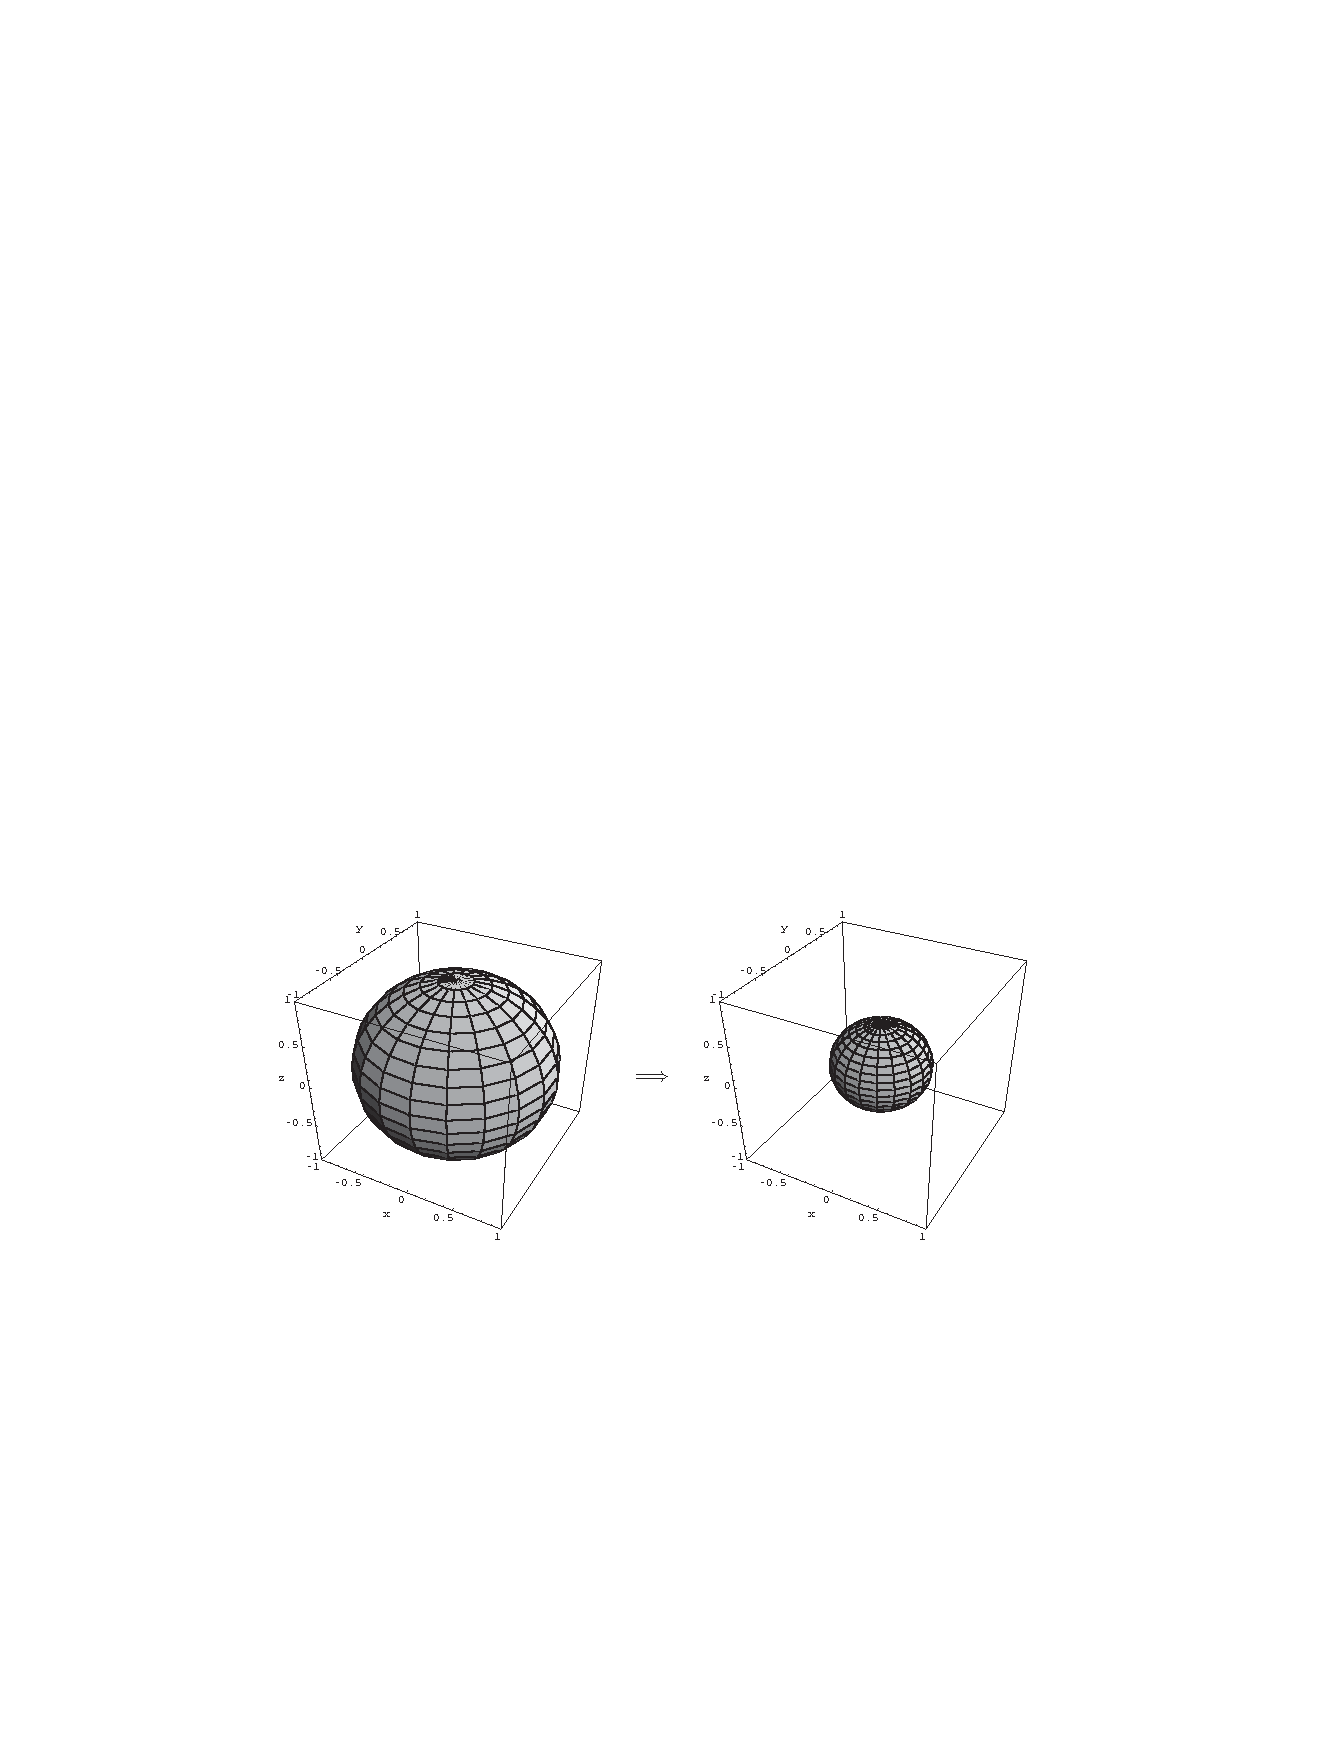
\includegraphics[width=15cm]{depolarizing-channel.pdf}
    \caption{Depolarizing channel~\cite{nielsen2010quantum}}
    \label{fig:depolarizing-channel}
\end{figure}

$n$ 量子ビットに対する Depolarizing チャネルは、次のように定義される。
\begin{align}
    \calN_p(\rho) = (1 - p)\rho + p\,\frac{\bbid}{2^n}
\end{align}
% これは、各量子ビットに対して Depolarizing チャネルを作用させることとは異なる。

\subsection*{Depolarizing チャネルによる量子ノイズモデル}
量子コンピューター上で、$n$ 量子ビットの初期状態 $\rho$ に対して、$L$ 個のユニタリ演算子を作用させることを考える。このとき、各ユニタリ演算子に付随して、Depolarizing チャネル $\calN_{p_i}$ が作用すると仮定する。作用させるユニタリチャネルを $\calE_i(\rho) = U_i\rho U_i\dg,\, i = 1,\,2,\,\cdots,\,L$ とすると、全体のチャネル $\calN$ は次のように表される。
\begin{align}
    \calN(\rho) = \qty(\bigcirc_{i=1}^L \calN_{p_i} \circ \calE_i)(\rho)
\end{align}
ここで、次のように $\calN_{p_i} \circ \calE_i = \calE_i \circ \calN_{p_i}$ が成り立つ。
\begin{align}
    \calN_{p_i} \circ \calE(\rho)
    = (1-p_i)(U\rho U\dg) + p_i\,\frac{\bbid}{2^n}
    = U\qty((1-p_i)\rho + p_i\,\frac{\bbid}{2^n})U\dg
    = \calE \circ \calN_{p_i}(\rho)
\end{align}

よって、$\calE := \bigcirc_{i=1}^L \calE_i$,  $\calN_{\bs{p}}^L := \bigcirc_{i=1}^L \calN_{p_i},\; \bs{p} = (p_1,\,p_2,\,\cdots,\,p_L)$ とすると、
\begin{align}
    \calN
    = \bigcirc_{i=1}^L \calN_{p_i} \circ \calE_i
    = \qty(\bigcirc_{i=1}^L \calN_{p_i}) \circ \qty(\bigcirc_{i=1}^L \calE_i)
    = \calN_{\bs{p}}^L \circ \calE
\end{align}
となる。つまり、$\calN$ は、$\calE$ の後に $\calN_{\bs{p}}^L$ が作用することと同じである。
簡単のため、$p_i = p$ とすると、$\calN_p^L(\rho)$ は次のように計算される。
\begin{align}
    \calN_{\bs{p}}^L(\rho) = (1 - p)^L\rho + \{1 - (1 - p)^L\}\,\frac{\bbid}{2^n}
\end{align}

このとき、次の $\calN$ を得る。
\begin{align}
    \calN(\rho)
    = \calN_{\bs{p}}^L \circ \calE(\rho)
    = (1 - p)^L\calE(\rho) + \{1 - (1 - p)^L\}\,\frac{\bbid}{2^n}
\end{align}


